\documentclass{mproj}
\usepackage{graphicx}

\usepackage[hyphens]{url}
\usepackage{fancyvrb}
\usepackage[final]{pdfpages}
\usepackage{times}
\usepackage{longtable}
\setlength{\LTcapwidth}{\textwidth}

%\usepackage[nottoc,numbib]{tocbibind}
\usepackage[nottoc]{tocbibind}

% for alternative page numbering use the following package
% and see documentation for commands
%\usepackage{fancyheadings}


% other potentially useful packages
\usepackage{amssymb,amsmath}
\usepackage{booktabs}

% Makes citations, cross-references, TOC entries and URLs clickable.
% hyperref must be loaded last (or very nearly last) -- it redefines commands
% from other packages, so anything loaded after it can undo its work.
% hypertexnames=false suppresses a harmless "duplicate destination" warning
% caused by the title page resetting the page counter.
\usepackage[hidelinks,hypertexnames=false]{hyperref}
\usepackage{caption} 
\captionsetup[longtable]{font=normalsize}

%\usepackage{url}
%\usepackage{fancyvrb}
%\usepackage[final]{pdfpages}

\begin{document}

%%%%%%%%%%%%%%%%%%%%%%%%%%%%%%%%%%%%%%%%%%%%%%%%%%%%%%%%%%%%%%%%%%%
\title{Temporal vs Static Models for Depression Detection in Speech: A Comparison Across Segment Lengths in the Androids Corpus}
\author{Gaurav Mahender Sidana}
\date{11 September 2026}
\maketitle
%%%%%%%%%%%%%%%%%%%%%%%%%%%%%%%%%%%%%%%%%%%%%%%%%%%%%%%%%%%%%%%%%%%

%%%%%%%%%%%%%%%%%%%%%%%%%%%%%%%%%%%%%%%%%%%%%%%%%%%%%%%%%%%%%%%%%%%
\begin{abstract}
Depression patients often find it difficult to maintain long spoken interactions, making the amount of speech required for reliable automatic detection an important question. This dissertation investigates whether a temporal classifier such as a stacked Recurrent Neural Network adapted from prior work on speech-based attachment recognition can detect depression more reliably than static classifiers (Logistic Regression, Support Vector Machine) when working from short speech segments. The models were trained on IS09 acoustic features extracted over the Androids Corpus under a person-independent 5-fold protocol, and compared across segment lengths from 32 to 1024 frames. The RNN achieved its best performance at a segment length of 32 frames (accuracy 73.5\%, F1 71.4\%), outperforming the equivalent Logistic Regression baseline (accuracy 66.4\%, F1 68.6\%). However, a paired t-test found this difference was not statistically significant at any segment length, while most models performed significantly above a random baseline. Repeating the experiments on the unedited interview recordings, which also contain the interviewer's speech, left the segment-based comparison unchanged but substantially raised the performance of a Support Vector Machine trained on whole-recording averages. These findings indicate that, within this experimental setup, temporal modelling does not yield a statistically significant advantage over static classification, and that segment length and level of aggregation may matter more than the presence of sequence memory itself.
\end{abstract}
%%%%%%%%%%%%%%%%%%%%%%%%%%%%%%%%%%%%%%%%%%%%%%%%%%%%%%%%%%%%%%%%%%%

%%%%%%%%%%%%%%%%%%%%%%%%%%%%%%%%%%%%%%%%%%%%%%%%%%%%%%%%%%%%%%%%%%%
\educationalconsent

%%%%%%%%%%%%%%%%%%%%%%%%%%%%%%%%%%%%%%%%%%%%%%%%%%%%%%%%%%%%%%%%%%%

\newpage
%%%%%%%%%%%%%%%%%%%%%%%%%%%%%%%%%%%%%%%%%%%%%%%%%%%%%%%%%%%%%%%%%%%
\section*{AI Declaration}

Generative AI tools were used in the preparation of this dissertation in the following ways:

\begin{itemize}
  \item Correcting grammar, spelling, and phrasing in text that I had already written. The content, structure, and argument of every passage are my own.
  \item Checking that cited works exist as described and that their bibliographic details are accurate. All sources were located, read, and assessed by me.
  \item Restructuring and splitting my existing Jupyter notebooks into a modular form as the scope of the study grew, from a single audio condition to two, from a single segment length to a sweep across several, and from one classifier to multiple static baselines. The implementation, experimental design, and analysis are my own work, and AI assistance was limited to reorganising existing code for clarity and efficiency.
\end{itemize}

AI has been used in line with the University of Glasgow's policy on the use of artificial intelligence. It has not been used in the critical evaluation of my sources, or in the formation of my arguments, conclusions, or outputs.

%%%%%%%%%%%%%%%%%%%%%%%%%%%%%%%%%%%%%%%%%%%%%%%%%%%%%%%%%%%%%%%%%%%

\newpage
%%%%%%%%%%%%%%%%%%%%%%%%%%%%%%%%%%%%%%%%%%%%%%%%%%%%%%%%%%%%%%%%%%%
\section*{Acknowledgements}

I owe my greatest thanks to my supervisor, Professor Alessandro Vinciarelli. What I took from working with him was an insistence on depth: it was never enough to know that a method worked, I had to understand why it behaved as it did before the result meant anything. He was patient through the stages where my grasp of the work was still shallow, and he kept asking questions until it wasn't. The second thing I learned from him is that research is not a hunt for good numbers. He encouraged me to explore ideas without worrying about whether they would beat a benchmark, and to treat a result that fails to confirm what I expected as an outcome to be understood rather than a failure. That framing gave me the confidence to pursue the questions in this dissertation on their own terms, and I am grateful for his time and for the standard he set.

My thanks also go to Parth Shringarpur, a good friend and our class representative, whose willingness to advocate for the cohort made the year run more smoothly for all of us. His encouragement and good humour made the more demanding parts of the process easier to navigate. I am grateful too to my fellow dissertation students, whose readiness to share ideas, offer feedback, and discuss their own experiences made the process feel far less solitary. I would also like to thank the University of Glasgow and the School of Computing Science for the environment and resources that made this work possible.

Above all, I thank my mother. This degree exists because of what she gave up for it, and because she never treated it as anything other than worth doing. I am grateful as well to the rest of my family and to my friends, who kept me steady through a demanding year and reminded me there was a life running alongside it.

%%%%%%%%%%%%%%%%%%%%%%%%%%%%%%%%%%%%%%%%%%%%%%%%%%%%%%%%%%%%%%%%%%%
\tableofcontents
%%%%%%%%%%%%%%%%%%%%%%%%%%%%%%%%%%%%%%%%%%%%%%%%%%%%%%%%%%%%%%%%%%%

%%%%%%%%%%%%%%%%%%%%%%%%%%%%%%%%%%%%%%%%%%%%%%%%%%%%%%%%%%%%%%%%%%%
\chapter{Introduction}\label{intro}

Depressive disorder, commonly known as depression, is characterised by persistent low mood, loss of interest or pleasure, poor concentration, and feelings of guilt or worthlessness, together with a range of physical and cognitive symptoms that may persist for weeks or considerably longer \cite{who2026depression}. Its global burden is substantial and growing. The World Health Organization estimated that 280 million people, some 5\% of all adults, experienced depression in 2019 \cite{who2026depression}, and reported a 25\% rise in global anxiety and depression during the first year of the COVID-19 pandemic \cite{who2022covid}. By 2021 the number of cases had reached 332.4 million, and is projected to exceed 466 million by 2040 \cite{zhang2025burden}. Younger people bear a disproportionate share of this increase: data from the UK's COSMO study show that poor mental health among 16 and 17 year olds has risen by more than a quarter since 2017, with 44\% now reporting high levels of psychological distress, nearly double the rate recorded in 2007 \cite{cosmo2025}. Set against the limited capacity of traditional psychiatric assessment, these trends point to a need for automated systems capable of fast and accessible screening.

Automatic technologies offer one route to screening at this scale. The approaches proposed in the literature rely on the premise that depression produces observable, measurable changes in behaviour, in tone of voice, choice of words, and other everyday signals of expression, and that machine learning models can be trained to detect these changes. Within this body of work, speech is the most widely used source of depression traces. One reason is that speech carries both signal-level and content-level information in a single modality, spanning paralanguage and language. Another is practicality: speech is easy and unobtrusive to capture, requiring no specialised sensors, and can be recorded over a telephone call or a laptop microphone.

Standard methodologies in speech-based detection treat speech (or segments of it) as a static input: either a single feature vector or an aggregate computed over a fixed-length window, both of which collapse the sequence into a single snapshot. This is a curious simplification given that speech is inherently sequential (word order and prosodic contour unfold over time). This raises the question of whether static representations are sufficient or, whether they discard information that a temporal classifier could exploit. Recent work has shown that a stacked RNN architecture can achieve reliable performance, well above chance on related paralinguistic classification tasks such as attachment recognition from children's spontaneous speech \cite{alsofyani2021}, suggesting that temporal architectures are worth testing for depression detection specifically. Such architectures have been applied to this task before, but typically alongside richer feature representations than those given to the static systems they are compared against. Architecture and representation therefore vary together. The comparison under a matched representation, across a systematic range of segment lengths, has not to our knowledge been made.

This dissertation investigates whether a temporal classifier can detect depression more reliably from speech than static classifiers, and whether any advantage depends on the segment length of the speech provided. The Androids Corpus, a publicly available dataset of 116 participants (64 depressed and 52 control cases) recorded as clinical interviews, was used to compare the two approaches. The two approaches differ in the way they process information: one uses a static representation, while the other processes the data sequentially. Frame-level features are first extracted using OpenSMILE, then grouped into segments ranging from 32 to 1024 frames to test the effect of context length. Following this, the trained classifiers' predictions are aggregated using majority vote and weighted average to produce the final speaker-level label, and evaluated using accuracy and F1 score. Because each recording captures both the participant and the interviewer, all experiments are run twice: once over the participant's speech in isolation, which is the primary condition reported throughout, and once over the full recordings, to test whether the interviewer's presence changes the comparison. If the temporal classifier performs significantly better than the static baseline, this would indicate that it captures sequential information the static classifier ignores. A non-significant result, however, would be harder to interpret: given the size of the corpus, it could reflect either a genuine absence of advantage or insufficient statistical power to detect one. Chapter~\ref{conclusion} returns to this distinction.

The rest of the dissertation is organized as follows. Chapter~\ref{survey} reviews previous work on speech-based depression detection, including the architecture precedent this dissertation builds on. Chapter~\ref{architecture} describes the corpus, pipeline, architectures and evaluation protocol used in the experiments. Chapter~\ref{results} presents the experiment results and their implications. Chapter~\ref{conclusion} concludes with a summary of findings and their limitations.

%%%%%%%%%%%%%%%%%%%%%%%%%%%%%%%%%%%%%%%%%%%%%%%%%%%%%%%%%%%%%%%%%%%
\chapter{Survey}\label{survey}

This section reviews the body of work identifying measurable depression markers in speech, covering both acoustic and linguistic traces studied in the literature. While this dissertation focuses on the acoustic/paralinguistic channel, the following review situates that choice within the broader landscape of speech-based depression detection before turning, in Section 2.2, to how such markers have typically been modelled.

\section{Depression detection from speech}\label{sec:markers}

Speech has been established as a diagnostic and monitoring aid for depression across a substantial body of prior work \cite{cummins2015acoustic,cummins2015review,cummins2014ivectors,scherer2014audiovisual,williamson2014}. This is grounded in the idea that depression's effects on the speech production system leave measurable traces that can serve as an objective marker of the disorder \cite{morales2016}. These traces span both the timing and quality of vocal production, motivating a range of studies that isolate specific acoustic markers of depression. Experiments performed by Cannizzaro et al.\ \cite{cannizzaro2004} found a statistically significant correlation between depression and speech signals. In that study, acoustic measures of speaking rate and pitch variation were examined against depression severity as self-rated by seven patients. For a comprehensive review of speech-based depression and suicide-risk assessment, see Cummins et al.\ \cite{cummins2015review}. Formants and power spectral density are found to be the most discriminative features for distinguishing depressed and control speakers, in the work by France et al.\ \cite{france2000}, an experiment involving 115 speakers, where the analysis was performed separately for male and female speakers and the findings were consistent in both. Voice quality measures such as jitter (variation in timing or period length between speech cycles) and shimmer (variation in amplitude or intensity of vocal cord vibration) have also been reported as being different for depressed and non-depressed speakers \cite{vicsi2012}. Another important characteristic of depression is a smaller vowel space (frequency span determined by the first two formants). This is a robust measure of depressed speech irrespective of the gender, ethnicity, or educational background of an individual \cite{scherer2016vowel}. Including pauses and speaking rate measures in an existing feature set reduces depression classification error by around 50\% \cite{tao2020}. Moore et al.\ \cite{moore2008} combined voice quality, prosodic, spectral, and glottal features to classify the presence/absence of depression, and reported high classification accuracies, with performance differing between male and female speakers. Experiments in Ozdas et al.\ \cite{ozdas2004} also show that glottal flow spectrum allows one to distinguish between control, suicidal, and depressed speakers (this experiment involved 10 participants). The studies surveyed above, and several of the specific findings reported for them, are also discussed in the review of acoustic depression markers given by Alsarrani et al.\ \cite{alsarrani2025}. Despite the breadth of markers identified across this literature, the classical marker-oriented work surveyed above almost uniformly reduces each recording, or a fixed-length window of it, to a single static representation for classification. The next section examines that assumption, and the sequential alternatives that have since been proposed.

Beyond acoustic traces, depression is also understood to leave measurable signatures in language itself, a link supported by psychological theory as well as by direct empirical findings in textual data. Beck's \cite{beck1967} cognitive theory proposes that individuals prone to depression hold a depressive schema, which is a persistent tendency to interpret themselves, their circumstances, and the world in negative terms. This provides a theoretical basis for why depressed language differs systematically from non-depressed language rather than by chance. LIWC-based word counting \cite{tausczik2010} is the dominant method here, and its central result has been replicated widely: depressed individuals use more first-person singular pronouns and more negatively valenced terms, and fewer positive emotion words than controls \cite{rude2004}. While LIWC and related lexicon-based approaches remain the most widely used methods for detecting depression in language, they rely on fixed, hand-curated word categories and cannot capture context or word sense beyond term frequency. Consequently, recent work applies transformer-based models such as BERT \cite{senn2022}, which learn contextual representations and outperform static lexicons on classification tasks. Although multimodal models combining speech and text typically yield higher performance \cite{alhanai2018}, this dissertation focuses strictly on the acoustic and paralinguistic channel. Text-based linguistic markers are surveyed for context rather than being modelled.

\section{Static vs.\ Temporal Modeling of Speech}\label{sec:static-temporal}

Most traditional speech-based depression detection models convert audio recordings into fixed static summaries, such as global means or functional statistics of acoustic parameters, which are then evaluated via classifiers like Support Vector Machines or Logistic Regression \cite{cummins2014ivectors,moore2008}. While this is computationally efficient, it relies on the assumption that paralinguistic cues are uniform across the entire utterance. In clinical contexts, however, depression traces often manifest as momentary prosodic flatlining or varied pause durations rather than consistent global averages. Static aggregation also discards the temporal trajectory and time-varying prosodic shifts inherent to continuous speech, which sequence models are able to capture more effectively \cite{graves2013}.

By processing acoustic frames sequentially, Recurrent Neural Networks (RNNs) map the temporal evolution of a speaker's voice and preserve the contextual links between spoken segments and pauses. This makes them a plausible candidate for detecting the paralinguistic markers associated with depression. It is that expectation which the present work sets out to test rather than assume. To model these temporal dynamics, this work adopts a stacked RNN architecture following Alsofyani and Vinciarelli \cite{alsofyani2021}. Stacking recurrent layers allows the deeper layer to extract increasingly abstract representations of the sequence. Long unbroken sequences, however, give rise to vanishing and exploding gradients \cite{pascanu2013}. Alsofyani and Vinciarelli address this by splitting each recording into fixed-length segments, which confines backpropagation to a bounded number of steps. This avoids the gating mechanisms used by LSTM and GRU cells, keeping the recurrent cell simple. It also makes the amount of temporal context an explicit parameter of the model rather than a property of the recording. Their framework was validated for attachment classification in school-age children. Whether it transfers to depression, and how its behaviour depends on the segment length chosen, is the question taken up here.

Temporal architectures are not new to depression detection. Following early fully-connected networks, convolutional and recurrent models with LSTM units were shown to improve on static classifiers \cite{rejaibi2022,dumpala2021}. Sequence models operating jointly over audio and transcripts have also been applied to clinical interviews \cite{alhanai2018}. The amount of context supplied to such models has received attention as well. Dumpala et al.\ \cite{dumpala2021,dumpala2022} vary the number of contiguous segments given to an LSTM trained on speaker embeddings, from roughly twenty seconds up to the length of the shortest recording in the test set, and report that performance depends on the context length chosen. Closer to the present work, Alsarrani et al.\ \cite{alsarrani2022thin} apply thin slices theory to the corpus used here, segmenting each recording into short slices and showing that classification improves relative to treating the recording as a whole.

These studies establish both that temporal models perform well on depression detection and that context length matters. They leave open a narrower question. In each case the temporal model differs from its static comparison in more than architecture. It is usually given different input features as well, and often a different unit of speech to classify. A model that reads speaker embeddings sequentially, for example, is compared against a Support Vector Machine reading simple averages of acoustic measurements, so an improvement could come from the better input rather than from the sequential reading. The segmentation studies have the opposite limitation. They change how much speech a classifier receives without asking whether a model that reads it in order uses it any differently from one that does not.

\section{The Androids Corpus and Prior Benchmarks}\label{sec:corpus-survey}

The primary dataset used in this dissertation is the Androids Corpus, introduced by Tao, Esposito, and Vinciarelli \cite{tao2023androids}. It includes audio recordings for a reading task and an interview task collected from participants across mental health centers in Southern Italy. The interview task was specifically selected for model training because spontaneous speech more reliably captures the natural prosodic and paralinguistic variations associated with depression, which are often masked or suppressed during constrained reading tasks. The interview task subset used here comprises recordings from 116 participants, of which 64 are individuals diagnosed with depression by professional psychiatrists. This study utilizes the speaker-independent k-fold splits provided with the corpus to ensure fair cross-study evaluation. Multiple architectures have previously been tested on these specific splits, with Alsarrani et al.\ \cite{alsarrani2025} compiling F1 and accuracy results from these and other approaches in a comparative summary. To contextualize these results, a Support Vector Machine trained on whole-recording averages is also included as a reference point against the corpus baseline.

\section{The Gap}\label{sec:gap}

The literature reviewed above reveals a consistent pattern. Acoustic markers of depression are well documented, spanning voice quality, spectral structure and timing (Section 2.1), and temporal architectures have been applied to the task with success (Section 2.2). What has not been established is how much of that success is owed to sequence modelling itself. Prior comparisons vary architecture and input representation together, so the contribution of temporal capacity cannot be separated from that of the features it operates on. The interaction between the two has not been examined either. It remains unclear whether any advantage a temporal model holds depends on how much context it is given, and whether that dependence differs from a static classifier's.

This question is related to, but distinct from, two addressed by Alsarrani and colleagues. The first \cite{alsarrani2022thin} asks how brief a slice of behaviour can be and still permit detection, and answers it by segmenting recordings and aggregating over the resulting slices. Segment length there is a property of the data supplied to the classifier, and the classifiers compared are static. The second \cite{alsarrani2025} asks whether depression traces are punctual or continuous, comparing Single Instance Learning against Multiple Instance Learning. Multiple Instance Learning allows a minority of depression-indicative feature vectors to determine a segment's label, while Single Instance Learning requires a majority. Both are questions about the data and how it is aggregated. In contrast, this dissertation asks whether sequential memory, an architectural property rather than an aggregation rule, improves depression detection over static classification given identical features, and how that comparison varies with segment length.

A second question follows from the recordings themselves. The Androids interviews capture both participant and interviewer, and the corpus distributes participant-only clips alongside the unedited recordings. Published results do not always state which is used. Interviewers are known to modify their acoustic behaviour in response to a participant's depression severity \cite{scherer2014dyadic}, and Watawana et al.\ \cite{watawana2026} show on this corpus that models trained on interviewer speech alone can match those trained on participant speech. Their analysis is confined to the text modality, and they identify the acoustic case as future work. Whether the choice of audio condition affects the temporal-versus-static comparison is therefore examined here as a second question.

To address these questions, this dissertation compares a stacked Recurrent Neural Network against static Logistic Regression and Support Vector Machine baselines, all trained on an identical feature representation, across a systematic range of segment lengths and under both audio conditions of the Androids Corpus.

%%%%%%%%%%%%%%%%%%%%%%%%%%%%%%%%%%%%%%%%%%%%%%%%%%%%%%%%%%%%%%%%%%%
\chapter{Architecture}\label{architecture}

The pipeline follows four main steps: feature extraction, segmentation, classification, and aggregation, illustrated in Figure~\ref{fig:pipeline}. In the first step, audio recordings are converted into sequences of feature vectors. In the segmentation step, each sequence is split into fixed-length segments of $L$ vectors. In the third step, each segment is assigned to the depressed or control class. In the final step, the resulting segment-level predictions are aggregated into a single speaker-level label.

\begin{figure}[htbp]
  \centering
  \includegraphics[width=\textwidth]{figures/pipeline_overview}
  \caption{The processing pipeline. Feature extraction converts each recording
  into a sequence of frame-level vectors, which is divided into non-overlapping
  segments of $L$ frames. Every segment is classified by a stacked RNN and,
  independently, by a Logistic Regression, and the resulting segment-level
  outcomes are combined into a speaker-level label by majority vote or weighted
  average. The Support Vector Machine (shown in red) bypasses segmentation
  entirely, averaging all frames of the recording into a single vector.}
  \label{fig:pipeline}
\end{figure}

\section{Feature Extraction}\label{sec:features}

Frame-level acoustic features are extracted from each recording using OpenSMILE \cite{eyben2013}, following the same feature extraction configuration used by Alsofyani and Vinciarelli \cite{alsofyani2021} for attachment recognition from children's spontaneous speech, the architectural precedent this dissertation adapts (Section 2.2). Features are computed over non-overlapping analysis windows of 33\,ms, with feature values smoothed by averaging across three consecutive windows. The smoothing is applied as a moving average and does not decimate the sequence, so the frame period remains 33\,ms and a segment of $L$ frames spans approximately $33L$\,ms. The feature set comprises 16 basic features: Root Mean Square Energy (1 feature), Mel Frequency Cepstral Coefficients (12 features), Zero Crossing Rate (1 feature), Voicing Probability (1 feature), and Fundamental Frequency (1 feature), each paired with its corresponding delta (first-order derivative) coefficient, giving a total feature dimensionality of $D = 32$. These features are consistent with those established in the literature as effective markers of voice quality and prosody relevant to depression (Section 2.1). The same representation is used for every model evaluated in this work, so that any performance difference observed between the temporal and static classifiers can be attributed to the architecture itself rather than to differences in the underlying features.

For a given recording, the result of this process is a sequence of feature vectors $X = (\vec{x}_1, \vec{x}_2, \ldots, \vec{x}_T)$, where $\vec{x}_t$ denotes the feature vector extracted at frame $t$, and $T$ is the total number of frames extracted from that recording (Figure~\ref{fig:pipeline}).

Feature extraction is performed twice, once for each audio condition. The primary condition uses the participant-only clips distributed with the corpus, concatenated in chronological turn order to give one sequence per speaker. The secondary condition uses the full interview recordings, which also contain the interviewer's voice, and serves as a check on whether the interviewer's presence affects the comparison.

\section{Segmentation}\label{sec:segmentation}

Training a recurrent model over long, unbroken sequences gives rise to vanishing and exploding gradients \cite{pascanu2013}. Alsofyani and Vinciarelli \cite{alsofyani2021} address this by splitting each recording into fixed-length segments of $L = 128$ frames before training, corresponding to approximately 4.25 seconds of speech under their windowing configuration. Since this dissertation's central question concerns how classifier performance depends on the amount of temporal context provided, segment length itself is treated as an independent variable rather than fixed at a single value: each recording's feature sequence $X$ is divided into non-overlapping segments across six lengths, $L \in \{32, 64, 128, 256, 512, 1024\}$ frames, equivalent to approximately 1.1 to 33.8 seconds of speech, spanning roughly two orders of magnitude from a few seconds of speech to durations approaching that of a full recording.

For a recording of length $T$, the number of complete segments at a given length $L$ is $M = \lfloor T / L \rfloor$. Any remaining frames that do not fill a complete final segment are discarded, ensuring that every segment used in training and evaluation contains exactly $L$ frames. Each classifier (Section 3.3) is trained and evaluated separately at every segment length, allowing the effect of context length on classification performance to be observed directly.

\section{Classification: Model Architectures}\label{sec:models}

Each segment is classified independently by one of two models: a temporal classifier (a stacked Recurrent Neural Network) or a static classifier (Logistic Regression), trained on an identical feature pipeline to isolate architecture as the variable under test. Because a recording yields many segments, the segment-level outcomes of both models are combined into a speaker-level label by two aggregation strategies, described in Section 3.4: a majority vote over the segments, and a weighted average of their predicted probabilities. Both strategies are applied to both classifiers, so that architecture and aggregation vary independently of one another. A third model, a Support Vector Machine, is evaluated separately under a different aggregation strategy, following the approach used in the corpus's original benchmark, and serves as a reference point rather than as a matched comparison.

\textbf{Temporal classifier (RNN).} Following Alsofyani and Vinciarelli \cite{alsofyani2021}, a stacked RNN with two layers processes each segment's sequence of feature vectors $\vec{x}_t$, using the hyperbolic tangent (tanh) activation function. At each frame $t$, the first layer produces a hidden state $\vec{h}_t$, which is passed as input to the second layer to produce a further hidden state $\vec{h}\,'_t$. Stacking layers in this way allows the deeper layer to extract increasingly abstract representations of the sequence (Section 2.2). Both layers use a hidden state dimension of 70. The final hidden state $\vec{h}\,'_L$, corresponding to the last frame of the segment, is passed through a single output unit, producing a logit that is converted by the logistic function into the posterior probability of class depressed. The segment is assigned to that class when this probability exceeds 0.5.


\textbf{Static classifier (Logistic Regression).} For comparison, a Logistic Regression classifier is trained on the same frame-level feature vectors, without access to their sequential structure. Each vector $\vec{x}_t$ is classified independently, yielding the posterior probability that that frame belongs to the depressed class. The segment is assigned to the depressed class when the majority of its $L$ frames are individually assigned to it.

\textbf{Static reference point (Support Vector Machine).} A Support Vector Machine is trained on whole-recording, speaker-level feature vectors, obtained by averaging all frame-level features for a given speaker into a single vector, following the aggregation strategy used in the corpus's original benchmark \cite{tao2023androids}. Unlike the comparison between the RNN and Logistic Regression, which is evaluated across all six segment lengths, this model uses the full recording as its unit of context and is evaluated once, providing a point of comparison against previously published results on the corpus rather than against the segment-length sweep itself.

\section{Aggregation}\label{sec:aggregation}

Since the RNN and Logistic Regression classifiers both operate at the level of individual segments, a recording divided into $M$ segments produces $M$ segment-level predictions that must be combined into a single speaker-level label. Two aggregation strategies are applied to both classifiers. The first, majority vote, assigns the speaker to the class their segments are most frequently classified as:
%
\begin{equation}
\hat{c} \;=\; \operatorname*{arg\,max}_{c \in \{c_1, c_2\}} f(c),
\end{equation}
%
where $f(c)$ is the fraction of segments assigned to class $c$ \cite{alsofyani2021}. The second, weighted average, instead averages the model's predicted probabilities across all $M$ segments before applying the 0.5 decision threshold once, at the speaker level. The two differ in the information they retain: the first discards the confidence of each segment-level decision, while the second preserves it.

The strategy in \cite{alsofyani2021} operates over two levels of aggregation, since each child in that work is represented by five separate story recordings. The Androids Corpus provides a single interview per speaker, so no intermediate level exists and the averaging is applied directly at the speaker level.

A consequence of this is that the Logistic Regression is, by construction, largely insensitive to $L$. Since each frame is classified in isolation, the segment length affects only how the frame-level probabilities are grouped before aggregation, and under the weighted average strategy the speaker-level score reduces to the mean probability over all frames of the recording irrespective of $L$. The Logistic Regression therefore acts as a length-invariant control: any variation in performance across segment lengths is attributable to the temporal model alone.

\section{Training and Evaluation Protocol}\label{sec:training}

Training and evaluation were performed according to a $k$-fold protocol ($k = 5$), using the folds provided with the Androids Corpus distribution (Section 4.1). The protocol is speaker-independent, so that no speaker appears in both the training and test sets of a given fold, ensuring that the models recognise depression rather than individual speakers. Features are standardised to zero mean and unit variance using statistics computed on the training fold alone, so that no information from the test fold influences training. For the RNN and Logistic Regression this standardisation is applied to the frame-level vectors, and for the Support Vector Machine to the speaker-level averages on which it operates.

The RNN is trained by minimising the binary cross-entropy between the estimated probability $\hat{y}$ and the true label $y \in \{0, 1\}$, which for a single segment is
%
\begin{equation}
\mathcal{L}(y, \hat{y}) \;=\; -\bigl[\, y \log \hat{y} + (1 - y) \log (1 - \hat{y}) \,\bigr],
\end{equation}
%
the negative log-likelihood of the label under a Bernoulli distribution with parameter $\hat{y}$. Parameters are updated with AdamW \cite{loshchilov2019}, a variant of Adam \cite{kingma2015} in which the shrinkage of parameters towards zero is separated from the gradient update. Adam scales each parameter's step by the inverse magnitude of its recent gradients, so an $L_2$ penalty added to the objective is scaled in the same way and regularises parameters unevenly according to their gradient history. AdamW instead subtracts the decay term directly after the adaptive step, shrinking every parameter by the same proportion. The learning rate is $1 \times 10^{-4}$, the decay coefficient $1 \times 10^{-2}$, and training proceeds for 30 epochs over mini-batches of 512 segments.

Two further measures address behaviour observed during cross-validation. Dropout is applied to the hidden states passed from the first recurrent layer to the second, each coordinate being set to zero with probability 0.3 during training, so that the second layer cannot come to depend on any individual coordinate. Gradient clipping bounds the size of any single update: whenever the norm $\|g\|$ of the gradient exceeds 5.0, the gradient is replaced by $5.0 \cdot g / \|g\|$, preserving its direction while preventing an occasional large gradient from displacing the parameters far from a region of low loss. While the architecture follows \cite{alsofyani2021}, these training choices were made independently and selected through cross-validation on the training folds.

Because the network's weights are initialised at random, its performance varies between training runs. Each configuration is therefore trained $R = 5$ times with different initialisations, following \cite{alsofyani2021} and \cite{alsarrani2025}, and the value recorded for each fold is the mean over the five repetitions. The Logistic Regression and Support Vector Machine are deterministic and are trained once per fold.

\section{Statistical Analysis}\label{sec:stats}

Performance is reported in terms of accuracy, precision, recall and F1 score, with F1 taken as the primary metric given the class imbalance of the corpus. Since the corpus provides the gender of every speaker, all metrics are additionally reported separately for female and male participants. All models are compared against a random baseline, which assigns each speaker to a class according to the class priors and whose expected performance is estimated over 1000 simulated trials.

Because the RNN is repeated across initialisations while the static classifiers are deterministic, the repetitions are averaged within each fold before any comparison is made. All reported standard deviations and all statistical comparisons are therefore computed over the five folds, so that the variance under test reflects variation across subsets of speakers rather than across random initialisations. Bouthillier et al.\ \cite{bouthillier2021} show that variance due to data sampling is substantially larger than variance due to weight initialisation, and that comparisons resting on the latter alone are the least reliable of the commonly used estimators. This departs from the practice in \cite{alsofyani2021} and \cite{alsarrani2025}, where comparisons are made across repetitions. Those comparisons are between models of the same type, whereas the comparison of interest here is between a stochastic and a deterministic classifier, for which initialisation variance is not an appropriate reference.

Comparisons between models are made with two-tailed paired $t$-tests across folds. Pairing is appropriate because every model is evaluated on the identical folds and the identical speakers, so fold-to-fold variation is shared between the two models being compared and can be removed. Comparisons against the random baseline are made with one-tailed single-sample $t$-tests, since only an improvement over chance is of interest.

Two families of comparisons are performed at each segment length. The first tests the temporal classifier against the static classifier under a matched aggregation strategy, comprising two comparisons and giving a Bonferroni-corrected threshold of $\alpha = 0.025$. The second tests each model and aggregation combination against the random baseline, comprising four comparisons and giving $\alpha = 0.0125$. The comparison between the two audio conditions (Section 4.3) forms a third family of four comparisons per segment length, again at $\alpha = 0.0125$.

With only five folds these tests have limited statistical power. A non-significant result therefore indicates that a difference could not be detected at this sample size, not that no difference exists, and this distinction is observed throughout the interpretation of the results.

\section{Reproducibility}\label{sec:reproducibility}

All experiments were implemented in Python 3.12 and can be reproduced from the code submitted alongside this dissertation. Acoustic features were extracted with the openSMILE Python interface (2.6.0) \cite{eyben2013}. The recurrent models were implemented in PyTorch (2.11.0, CUDA 12.8), and the Logistic Regression and Support Vector Machine in scikit-learn (1.9.0), with NumPy 2.4.0, SciPy 1.18.0 and pandas 3.0.3 supporting data handling and the statistical tests. The complete environment, including all transitive dependencies and their exact versions, is provided as a conda environment file with the submitted code.

The five repetitions of each RNN configuration described in Section~\ref{sec:training} use fixed random seeds 0 to 4, which determine weight initialisation, dropout masks and mini-batch ordering, so that the reported means and standard deviations can be reproduced exactly. The fold assignments are those distributed with the corpus and are not regenerated. Training was performed on a single NVIDIA GeForce RTX 4060, and a complete sweep over all six segment lengths, five folds and five repetitions takes approximately 15 minutes under the participant-only condition and 20 minutes under the full-recording condition.

%%%%%%%%%%%%%%%%%%%%%%%%%%%%%%%%%%%%%%%%%%%%%%%%%%%%%%%%%%%%%%%%%%%
\chapter{Experiments and Results}\label{results}

This section describes the data used in the experiments (Section 4.1), reports the comparison between temporal and static classifiers across segment lengths (Section 4.2), and examines whether the conclusions hold when the interviewer's speech is included (Section 4.3).

\section{The Data}\label{sec:data}

All experiments were conducted on the interview task of the Androids Corpus \cite{tao2023androids}, described in Section 2.3. The interviews were recorded in standard clinical consultation rooms using a laptop microphone placed between the participant and interviewer, approximating realistic deployment conditions for a screening tool. Every interview followed the same sequence of questions about everyday life, and interviewers were instructed to minimise prompting. The reading task available in the corpus was not used, since spontaneous speech has been reported to yield more reliable depression detection than read speech \cite{alghowinem2013}.

\begin{table}[htbp]
  \centering
  \caption{Demographic composition of the Androids Corpus. Acronyms F and M
  stand for female and male, respectively.}
  \label{tab:demographics}
  \begin{tabular}{lcccc}
    \toprule
    Group     & F  & M  & Avg. Age        & Age Range \\
    \midrule
    Depressed & 43 & 21 & $47.5 \pm 11.6$ & 19--68 \\
    Control   & 41 & 11 & $47.3 \pm 12.7$ & 22--71 \\
    \midrule
    Total     & 84 & 32 & $47.4 \pm 12.1$ & 19--71 \\
    \bottomrule
  \end{tabular}
\end{table}

\begin{figure}[htbp]
  \centering
  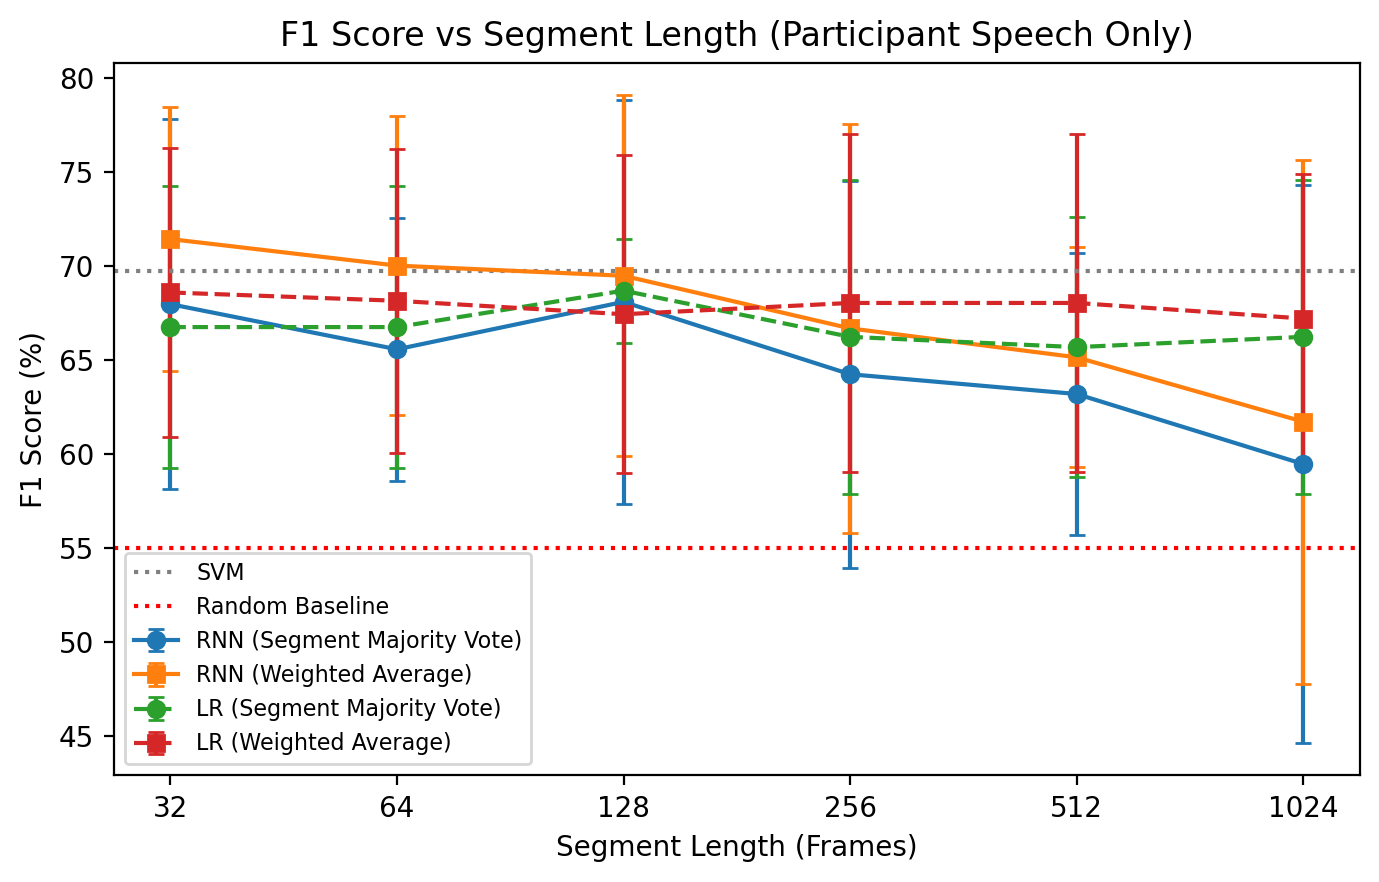
\includegraphics[width=0.92\textwidth]{figures/f1_score_vs_segment_length_participant_speech_only}\\[1.5ex]
  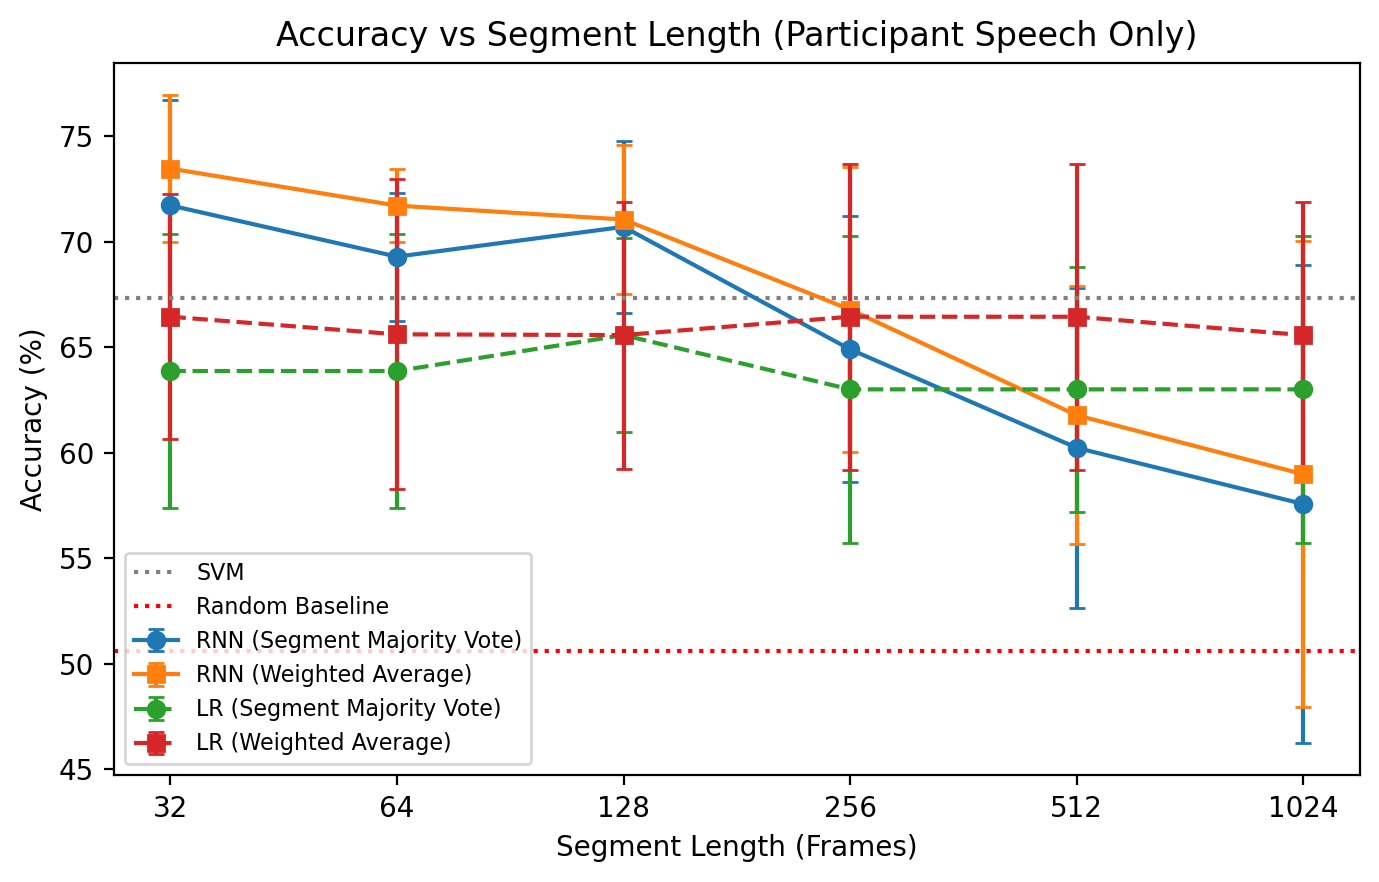
\includegraphics[width=0.92\textwidth]{figures/accuracy_vs_segment_length_participant_speech_only}
  \caption{F1 score (top) and accuracy (bottom) as a function of segment
  length, for the participant-only condition. Error bars show the standard
  deviation over the five folds. The Support Vector Machine and random baseline
  are shown as horizontal lines, since neither depends on segment length.}
  \label{fig:segment-length-participant}
\end{figure}

The corpus comprises 116 interviews from unique participants, of whom 64 were diagnosed with depression by professional psychiatrists according to DSM-5 criteria \cite{dsm5} and 52 had no history of mental health problems. Table~\ref{tab:demographics} summarises the demographic composition. The two groups are closely matched in age, with mean ages of 47.5 and 47.3 years and comparable spread, while both are predominantly female. Within the depressed group women outnumber men by roughly two to one (43 vs.\ 21), consistent with epidemiological observations that women experience depression roughly twice as frequently as men \cite{kessler2003}. The age range of both groups corresponds to the period in which depression most commonly develops \cite{kessler2003}.

\begin{table}[htbp]
  \centering
  \caption{Composition of the five person-independent folds distributed with
  the corpus.}
  \label{tab:folds}
  \begin{tabular}{lccc}
    \toprule
    Fold & Depressed & Control & Total \\
    \midrule
    1 & 12 & 12 & 24 \\
    2 & 13 & 10 & 23 \\
    3 & 10 & 13 & 23 \\
    4 & 18 &  5 & 23 \\
    5 & 11 & 12 & 23 \\
    \midrule
    Total & 64 & 52 & 116 \\
    \bottomrule
  \end{tabular}
\end{table}

All experiments follow the five person-independent folds distributed with the corpus, allowing direct comparison against previously published work on the same data. Table~\ref{tab:folds} gives the composition of each fold. The folds are of comparable size, containing between 23 and 24 speakers each, but differ considerably in class balance. Folds 1, 3 and 5 are close to even, whereas fold 4 contains 18 depressed and only 5 control speakers. This imbalance has a visible effect on the metrics: every segment-based model achieves 100\% precision on fold 4, since the number of possible false positives is bounded by the small size of the control group. The large precision standard deviations reported in Section 4.2 are attributable almost entirely to this fold.

Because the amount of speech available per speaker differs between the two audio conditions, recording durations were examined separately for each. Under the participant-only condition the mean duration is 176.4 seconds for depressed participants compared to 207.9 seconds for control participants (two-tailed $t$-test: $t = -2.03$, $p = 0.044$). The depressed group is also far more variable (standard deviations of 103.1 vs.\ 47.3 seconds), and excluding outliers beyond 1.5 times the interquartile range widens the difference considerably, to 157.3 vs.\ 204.4 seconds ($t = -4.24$, $p < 0.001$). In the full-recording condition, this gap widens to 198.8 vs.\ 268.0 seconds ($t = -4.65$, $p < 0.001$), reflecting the additional interviewer speech present in those recordings.

This duration difference reflects the pathology rather than a flaw in the data. Reduced verbal output is a documented feature of depression, associated with psychomotor retardation \cite{buyukdura2011}, and slower speech and shorter utterances have been reported to vary with depression severity \cite{mundt2012}. The segmentation procedure described in Section 3.2 nonetheless limits the influence of duration on classification, by aggregating over fixed-length segments rather than over any quantity that scales with total recording length.

\section{Depression Detection Results}\label{sec:detection-results}

This section reports the comparison between the temporal and static classifiers across segment lengths, using the participant-only condition described in Section 4.1. All results are obtained under the five person-independent folds distributed with the corpus, and F1 score is treated as the primary metric throughout, since the corpus contains more depressed than control participants (64 against 52) and accuracy alone is therefore a weak summary of performance. Table~\ref{tab:best-configs} reports the best configuration of each model, and Figure~\ref{fig:segment-length-participant} shows the variation of F1 score and accuracy with segment length. The complete set of results is given in Appendix~\ref{app:full-results}.

\begin{table}[htbp]
  \centering
  \small
  \setlength{\tabcolsep}{3.5pt}
  \caption{Best configuration of each model under both audio conditions. All
  values are percentages, reported as the mean and standard deviation over the
  five folds. Female and male F1 are computed over all speakers of each gender
  pooled across folds, and are therefore reported without standard deviations.
  The Support Vector Machine uses the whole recording as its unit of context
  and so has no associated segment length.}
  \label{tab:best-configs}
  \begin{tabular}{llccccrr}
    \toprule
    Model & $L$ & Acc. & Prec. & Rec. & F1 & F1$_{\text{F}}$ & F1$_{\text{M}}$ \\
    \midrule
    \multicolumn{8}{l}{\textit{Participant speech only}} \\
    SVM       & --  & $67.3 \pm 7.9$ & $68.7 \pm 14.9$ & $72.3 \pm 11.0$ & $69.7 \pm 10.6$ & 69.8 & 73.9 \\
    LR (SMV)  & 128 & $65.6 \pm 4.6$ & $71.1 \pm 17.6$ & $70.2 \pm 9.9$  & $68.7 \pm 2.8$  & 64.1 & 76.0 \\
    LR (WA)   & 32  & $66.4 \pm 5.8$ & $70.6 \pm 17.9$ & $68.7 \pm 5.8$  & $68.6 \pm 7.7$  & 64.9 & 76.0 \\
    RNN (SMV) & 128 & $70.7 \pm 4.1$ & $78.5 \pm 12.8$ & $60.7 \pm 10.4$ & $68.1 \pm 10.8$ & 63.8 & 80.4 \\
    RNN (WA)  & 32  & $73.5 \pm 3.5$ & $85.1 \pm 11.4$ & $63.5 \pm 10.7$ & $71.4 \pm 7.0$  & 67.2 & 81.9 \\
    \midrule
    \multicolumn{8}{l}{\textit{Full interview recording}} \\
    SVM       & --  & $80.2 \pm 4.9$ & $80.9 \pm 11.2$ & $82.8 \pm 6.3$  & $81.4 \pm 6.7$  & 78.0 & 89.4 \\
    LR (SMV)  & 32  & $62.1 \pm 10.9$& $74.1 \pm 21.8$ & $54.5 \pm 10.1$ & $60.9 \pm 9.9$  & 48.5 & 78.3 \\
    LR (WA)   & 32  & $64.7 \pm 9.3$ & $76.6 \pm 18.8$ & $55.6 \pm 8.1$  & $63.2 \pm 7.9$  & 52.3 & 78.3 \\
    RNN (SMV) & 32  & $77.2 \pm 3.8$ & $94.8 \pm 5.9$  & $62.6 \pm 6.7$  & $74.7 \pm 3.3$  & 68.5 & 86.9 \\
    RNN (WA)  & 32  & $77.4 \pm 2.6$ & $92.5 \pm 6.4$  & $64.2 \pm 7.1$  & $75.1 \pm 4.8$  & 69.4 & 87.4 \\
    \bottomrule
  \end{tabular}
\end{table}

The best performance overall is obtained by the RNN under Weighted Average at a segment length of 32 frames, reaching an accuracy of 73.5\% and an F1 score of 71.4\%. The corresponding Logistic Regression configuration reaches 66.4\% accuracy and 68.6\% F1, and the Support Vector Machine, operating on whole-recording averages, reaches 67.3\% and 69.7\%. All three therefore fall within roughly three F1 points of one another, despite differing substantially in the amount of context each uses and in whether that context is modelled sequentially.

The effect of segment length is the clearest pattern in the results. The RNN performs best at the shortest length tested and declines monotonically as segments lengthen: under Weighted Average its F1 score falls from 71.4\% at $L = 32$ to 61.7\% at $L = 1024$, with accuracy falling over the same range from 73.5\% to 59.0\%. The Logistic Regression, by contrast, is essentially flat, varying between 68.6\% and 67.2\% across all six lengths. This is the behaviour anticipated in Section 3.4: because the Logistic Regression classifies each frame in isolation, segment length affects only how frame-level probabilities are grouped before aggregation. The control therefore behaves as designed, and the entire observed effect of segment length is attributable to the temporal model.

This decline is likely driven by two factors. The first concerns aggregation rather than modelling: as $L$ grows, each speaker yields proportionally fewer segments, so the aggregation step operates over fewer predictions and the speaker-level decision becomes correspondingly less stable. The second concerns the model itself, since a recurrent network with tanh activations must carry information across increasingly long sequences, which is precisely the difficulty that motivated segmentation in the first place (Section 3.2). The results at $L = 1024$ are consistent with both: the F1 score of 61.7\% is accompanied by a standard deviation of 13.9 points, the largest of any configuration tested, indicating that performance at this length depends heavily on which speakers fall in the test fold.

Turning to the central question, no statistically significant difference is observed between the temporal and static classifiers at any segment length, under either aggregation strategy. The largest difference in favour of the RNN occurs at $L = 32$ under Weighted Average, where its F1 score exceeds that of the Logistic Regression by 2.84 points, but this is not statistically significant ($t = 1.18$, $p = 0.303$; $\alpha = 0.025$). At the two shortest lengths the difference favours the RNN, and at $L \geq 256$ it reverses sign, with the Logistic Regression ahead by 1.35 and 2.89 points at $L = 256$ and $L = 512$ respectively. Therefore, under these conditions, a temporal classifier does not significantly outperform a static one. As noted in Section 3.6, the limited number of folds means that a difference of this size would not reliably be detected even if it were real, and the absence of a significant result should not be read as evidence that no such difference exists.

Although the two classifiers achieve comparable F1 scores, they arrive at them differently. At $L = 32$ the RNN achieves a precision of 85.1\% with a recall of 63.5\%, while the Logistic Regression achieves 70.6\% precision with 68.7\% recall. The temporal model is therefore markedly more conservative, assigning the depressed class less often but being correct more frequently when it does. A recall of 63.5\% means that roughly a third of depressed participants are classified as control. In clinical screening applications, false negatives carry the greater cost, since patients who need treatment are not identified. Recall is therefore typically prioritised.

Comparisons against the random baseline are less consistent than the mean scores alone would suggest. The Logistic Regression exceeds chance to a statistically significant extent at $L = 32$ and $L = 64$ under both aggregation strategies, and also at $L = 128$ under Segment Majority Vote and at $L = 1024$ under Weighted Average. The result at $L = 128$ under Segment Majority Vote is the strongest margin over chance recorded in this condition ($p = 0.0002$). The RNN under Weighted Average exceeds chance at $L = 32$, $L = 64$ and $L = 512$, while the RNN under Segment Majority Vote does not clear the corrected threshold at any length. The Support Vector Machine also exceeds chance ($p = 0.0179$), despite using no segmentation at all. With the exception of the Logistic Regression at $L = 128$, the $p$-values lie close to the corrected significance threshold, so fold-to-fold variance dictates the statistical outcome more than the absolute effect size. These comparisons should therefore be read as indicating that all configurations perform above chance to a broadly similar degree, rather than as separating them.

The Support Vector Machine, which uses the full recording as its unit of context, achieves an F1 score of 69.7\%, between the best Logistic Regression and the best RNN configurations. The difference between it and the best RNN is not statistically significant. Averaging over the whole recording therefore performs comparably to classifying fixed-length segments and aggregating the outcomes, which suggests that the information relevant to depression is distributed broadly enough across the recording that neither the temporal ordering of frames nor the choice of aggregation unit substantially alters what is recoverable.

Performance differs markedly between female and male speakers. Male F1 exceeds female F1 in every configuration tested, and often by a considerable margin: at $L = 32$ the RNN under Weighted Average achieves 81.9\% for male speakers against 67.2\% for female speakers, and the Logistic Regression achieves 76.0\% against 64.9\%. This is not explained by the amount of training material available, since female participants constitute 72\% of the corpus and are therefore the better-represented group. A difference in the same direction has been reported for unimodal approaches based on speech signals on this corpus \cite{alsarrani2025}, and one possible explanation is that the acoustic markers captured by the IS09 feature set are expressed more consistently in male speakers, though the present experiments cannot distinguish this from other explanations.

\begin{table}[htbp]
  \centering
  \caption{Results reported on the Androids Corpus. Figures for previous work
  are as reported in the comparative summary of Alsarrani et al.\
  \cite{alsarrani2025}; two further entries in that summary are omitted here,
  one because it does not report both metrics and one because it addresses a
  benchmarking question rather than depression detection performance. Not all
  works state whether they use the folds provided with the data, or which audio
  condition they use, but the values still provide a reference for comparison.}
  \label{tab:published}
  \begin{tabular}{lcc}
    \toprule
    Reference               & Accuracy (\%)   & F1 (\%) \\
    \midrule
    Baseline \cite{tao2023androids}        & $83.9 \pm 1.3$  & $84.7 \pm 0.9$ \\
    Alsarrani et al.\ \cite{alsarrani2025} & $92.5 \pm 1.1$  & $93.1 \pm 1.1$ \\
    Ilias and Askounis \cite{ilias2024} & $95.3 \pm 4.2$  & $95.8 \pm 3.8$ \\
    Ntalampiras \cite{ntalampiras2025}        & $87.0 \pm 1.2$  & $88.9 \pm 1.7$ \\
    Phukan et al.\ \cite{phukan2024}     & 87.9            & 83.3 \\
    Yu and Kaya \cite{yu2025}         & $88.2 \pm 8.5$  & $86.3 \pm 11.5$ \\
    \midrule
    This work               & $73.5 \pm 3.5$  & $71.4 \pm 7.0$ \\
    \bottomrule
  \end{tabular}
\end{table}

Finally, the absolute performances reported here are lower than those published elsewhere on the Androids Corpus, as Table~\ref{tab:published} shows. The best F1 score obtained in this work, 71.4\%, is below the 84.7\% reported for the baseline distributed with the corpus \cite{tao2023androids} and well below the 93.1\% reported by Alsarrani et al.\ \cite{alsarrani2025}. Those systems use richer representations and more elaborate classification schemes, including self-supervised speech embeddings, multimodal fusion of speech signals with their transcriptions, and multiple instance learning. The present work instead holds the representation fixed at 32-dimensional IS09 features for every model, precisely so that architecture rather than representation is the variable under test. Maximising absolute performance is not the object of these experiments, and a system designed for that purpose would make different choices at every stage of the pipeline. Because the representation is held constant across every model compared, the relative comparison between temporal and static modelling remains valid despite the lower absolute ceiling.

Taken together, these results indicate that within this experimental setup the capacity to model temporal structure gives no measurable advantage over classifying frames independently. What does affect performance is the amount of context supplied to the temporal model and the way segment-level outcomes are aggregated: the RNN's best result is obtained at the shortest segment length tested, roughly one second of speech, and its performance degrades steadily as that context is extended.

\section{Effect of the Audio Condition}\label{sec:audio-condition}

All results reported so far use the participant-only condition. This section repeats the same experiments on the full interview recordings, which additionally contain the interviewer's speech, to determine whether the comparison between temporal and static classification depends on which audio is used. Table~\ref{tab:best-configs} reports the best configuration of each model under both conditions, and Figure~\ref{fig:segment-length-full} shows the variation of F1 score and accuracy with segment length for the full recordings.

\begin{figure}[htbp]
  \centering
  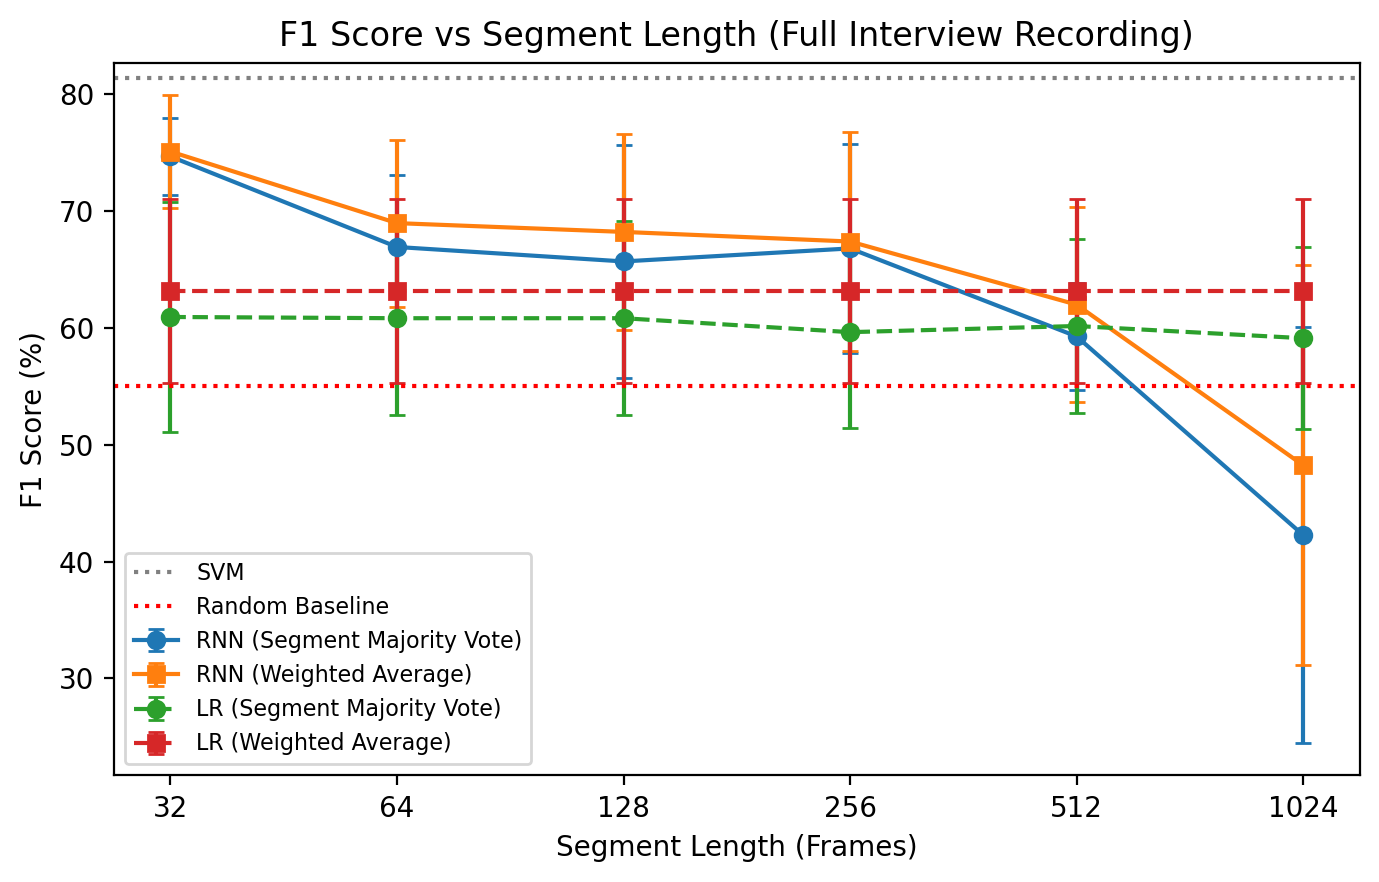
\includegraphics[width=0.92\textwidth]{figures/f1_score_vs_segment_length_full_interview_recording}\\[1.5ex]
  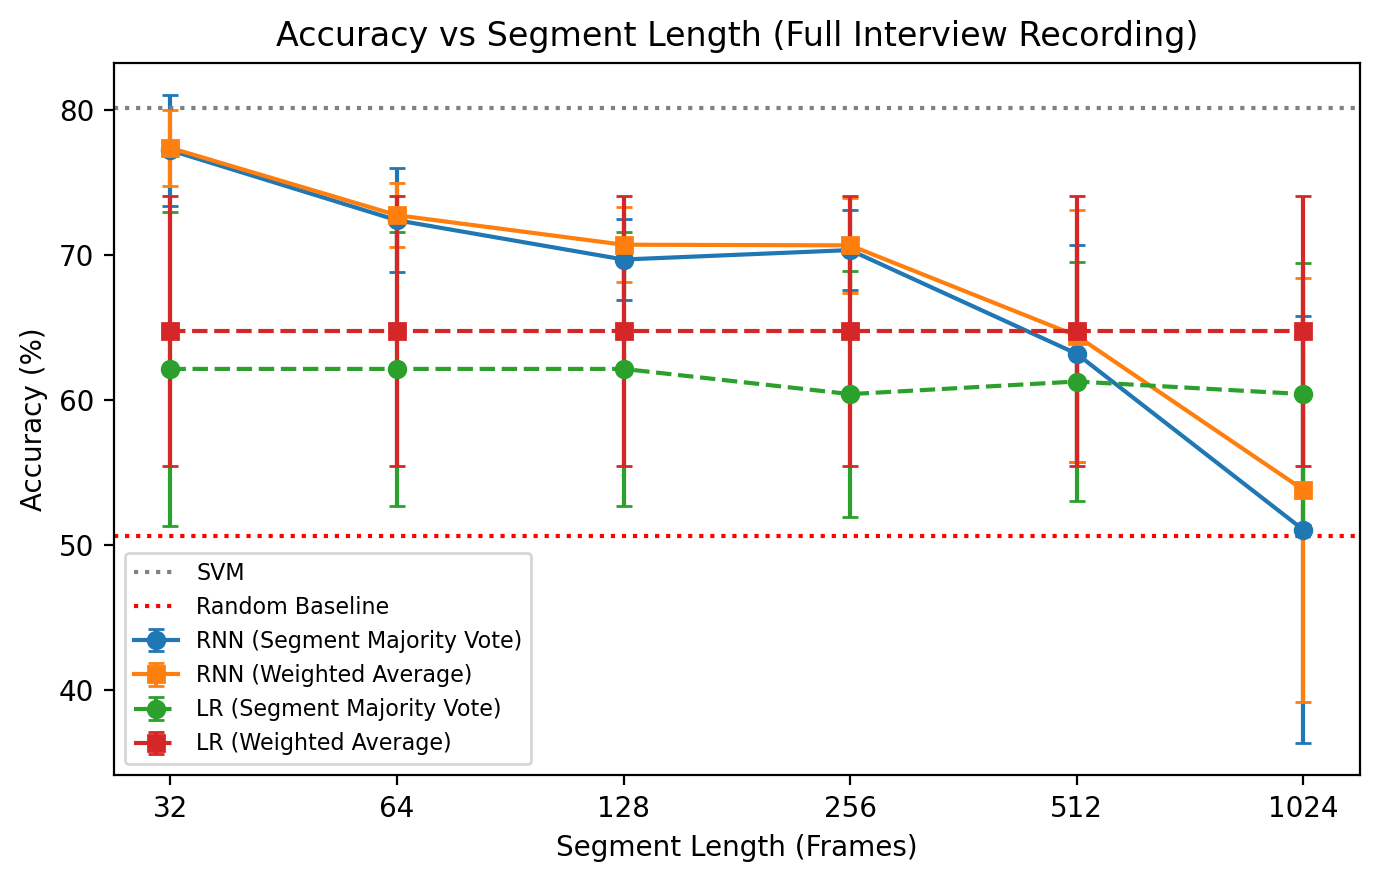
\includegraphics[width=0.92\textwidth]{figures/accuracy_vs_segment_length_full_interview_recording}
  \caption{F1 score (top) and accuracy (bottom) as a function of segment
  length, for the full interview recordings. Error bars show the standard
  deviation over the five folds. The Support Vector Machine and random baseline
  are shown as horizontal lines, since neither depends on segment length.}
  \label{fig:segment-length-full}
\end{figure}

The three models respond to the change in opposite directions. At $L = 32$, the RNN improves by 6.72 F1 points under Segment Majority Vote and 3.68 points under Weighted Average, while the Logistic Regression declines by 5.80 and 5.43 points respectively. None of these differences is statistically significant ($p = 0.1005$, $0.0781$, $0.2238$ and $0.2297$ against a corrected threshold of $\alpha = 0.0125$), and no comparison at any segment length reaches significance, the largest being a decline of 17.18 points for the RNN under Segment Majority Vote at $L = 1024$ ($t = -2.97$, $p = 0.0411$). The Support Vector Machine is affected most, improving from 69.7\% to 81.4\% F1 ($t = 2.78$, $p = 0.0499$). Since the interviewer's speech cannot carry the participant's own paralinguistic markers, none of these changes can be attributed to a better representation of the participant's voice.

The apparent advantage of the temporal classifier is considerably larger under this condition. At $L = 32$, the RNN exceeds the Logistic Regression by 13.74 F1 points under Segment Majority Vote and 11.94 points under Weighted Average, compared with 1.22 and 2.84 points respectively in the participant-only condition. Neither reaches significance at the corrected threshold ($p = 0.0386$ and $p = 0.0389$ against $\alpha = 0.025$), but both are considerably closer to it than any comparison in the primary condition. Relying solely on the full recordings would have substantially altered the conclusions of Section 4.2.

The comparisons against chance invert. In the participant-only condition, the Logistic Regression exceeds chance at several segment lengths under both aggregation strategies, while the RNN under Segment Majority Vote never clears the corrected threshold. In the full-recording condition, the Logistic Regression fails to exceed chance at any segment length under either strategy, while the RNN clears the threshold at $L = 32$ and $L = 64$ under both strategies by a wide margin, reaching $p = 0.0001$ under Segment Majority Vote at $L = 32$. The full recordings therefore help the temporal model and harm the static one.

The behaviour of precision is informative. Under the full recordings, the RNN's precision at $L = 32$ rises to 94.8\% under Segment Majority Vote and 92.5\% under Weighted Average, up from 85.1\% under both strategies in the participant-only condition. Recall, however, barely changes, remaining at 62.6\% and 64.2\% respectively, compared with 58.9\% and 63.5\%. The model becomes markedly more selective without identifying substantially more depressed participants, which is consistent with it exploiting some property that distinguishes the recordings themselves rather than a stronger signal of the pathology.

Several such properties are available in the full recordings. Section 4.1 shows that the duration difference between groups widens considerably once the interviewer's speech is included, from 31 seconds to 69 seconds. The recordings also contain turn structure, silence distribution and the interviewer's own speech, none of which is present in the participant-only condition. Interviewers are known to modify their acoustic behaviour in response to a participant's depression severity, and the degree of accommodation between the two speakers has been reported to vary inversely with severity \cite{scherer2014dyadic}. More directly, Watawana et al.\ \cite{watawana2026} show on this same corpus that models trained on interviewer speech alone can match or exceed those trained on participant speech, and attribute this to models exploiting the fixed structure of the interview rather than the participant's own language. Their analysis is restricted to the text modality, and they identify the extension of the same comparison to acoustic features as future work. The results reported here are consistent with the effect persisting in that modality.

These observations do not establish which property is responsible, and the present experiments were not designed to isolate it. They do, however, support the decision to treat the participant-only condition as primary. A result obtained from the full recordings cannot be attributed to the participant's paralinguistic behaviour, which is the primary focus of the literature surveyed in Section 2.1. Consequently, the widened gap between the temporal and static classifiers under this condition is more plausibly explained by the additional non-participant information available to the sequential model than by a genuine advantage in modelling depression.

One further difference is notable. The performance gap between female and male speakers widens considerably under the full recordings: the Logistic Regression under Weighted Average reaches 78.3\% F1 for male speakers against 52.3\% for female speakers, a difference of 26 points, compared with 11 points in the participant-only condition. The same caveat as in Section 4.2 applies, since male participants constitute only 32 of the 116 speakers.

%%%%%%%%%%%%%%%%%%%%%%%%%%%%%%%%%%%%%%%%%%%%%%%%%%%%%%%%%%%%%%%%%%%
\chapter{Conclusion}\label{conclusion}

This dissertation investigated whether a temporal classifier detects depression from speech more reliably than static classifiers trained on the same representation, and whether any such advantage depends on the amount of speech supplied. A stacked Recurrent Neural Network with non-gated recurrent units, adapted from prior work on attachment recognition in children, was compared against Logistic Regression and a Support Vector Machine over the Androids Corpus, with all models trained on an identical set of IS09 acoustic features under the five person-independent folds distributed with the corpus.

The temporal classifier achieved its best performance at the shortest segment length tested, approximately one second of speech, reaching 73.5\% accuracy and 71.4\% F1. This exceeded the matched Logistic Regression baseline by 2.84 F1 points, but the difference was not statistically significant at any segment length, under either aggregation strategy. Within this experimental setup, therefore, a simple recurrent architecture gave no measurable advantage over classifying frames independently. Two caveats attach to that conclusion. The first is its scope: it holds for one architecture, one feature representation and one corpus, and the decline observed at longer segment lengths is itself consistent with a limitation of non-gated recurrent units rather than of sequence modelling in general. The second is statistical: with only five folds, a difference of the size observed would not reliably have been detected even if it were real, and the absence of a significant result is not evidence that no difference exists.

However, the amount of supplied context markedly affected performance. The temporal model performed best on the shortest segments and declined steadily as they lengthened, while the static classifier, which is insensitive to segment length by construction, remained flat throughout. Since both models saw identical features and folds, this variation is attributable to the temporal model alone. The practical implication is a favourable one for the clinical setting that motivated this work: performance did not require long stretches of speech, and the best results were obtained from segments short enough that a brief interaction would suffice.

When repeated on the full interview recordings, the experiments demonstrated a larger apparent advantage for the temporal classifier, and a substantial improvement for the Support Vector Machine. Because the interviewer's speech cannot carry the participant's own paralinguistic markers, these gains are more plausibly explained by information about the recordings themselves than by a stronger signal of the pathology. This supports the decision to report the participant-only condition throughout, and indicates that results on this corpus depend on a choice of audio that published work does not always state.

Several limitations bear on these conclusions. The five folds provided with the corpus are unevenly balanced, and one contains only five control speakers, which inflates precision and widens the fold-to-fold variation on which every statistical comparison rests. Because the participant-only condition is constructed by concatenating individual turns, a segment may span a boundary that the model inaccurately treats as continuous speech. Male participants constitute only 32 of the 116 speakers and are unevenly distributed across folds, so the gender differences reported in Section 4.2 should be treated as indicative rather than established.

Beyond these, two decisions about the design of the study itself would be made differently with hindsight. Holding the feature set fixed at IS09 was necessary to isolate architecture, but it capped absolute performance well below what has been reported on this corpus, and starting from learned speech embeddings would have allowed the same comparison to be made at a more competitive level. The scope of the work also widened as it progressed: as properties of the corpus came to light, a substantial part of the effort went into establishing why the models behaved as they did rather than how well they performed. That shift was worthwhile, but it consumed time that would otherwise have gone to a comparison against gated recurrent architectures.

The null result was not the expected outcome, since a temporal model was anticipated to outperform frame-level classification. It has not changed what counts here as a finding, but it did make clear how much of the interpretation rests on the design of the comparison rather than on the numbers it produces.

Future research directions emerge from these limitations and from the reflections above. The two already identified, replacing handcrafted features with self-supervised speech embeddings and repeating the comparison with gated recurrent architectures, would together establish whether the null result reflects the architecture, the representation, or neither. Two further directions follow from the corpus itself. Confining segmentation within turns would remove the discontinuity introduced by concatenation, and the contribution of the interviewer, excluded from the primary condition here, is worth examining as a question in its own right, since the interviewer's behaviour may itself carry information about the participant's condition.

\appendix % first appendix
%%%%%%%%%%%%%%%%%%%%%%%%%%%%%%%%%%%%%%%%%%%%%%%%%%%%%%%%%%%%%%%%%%%
\chapter{Complete Results}\label{app:full-results}

This appendix reports the full set of results summarised in Chapter~\ref{results}. Tables~\ref{tab:appendix-metrics-participant} and~\ref{tab:appendix-metrics-full} give the classification metrics for every model and segment length under each audio condition. The remaining tables give the statistical comparisons, organised by the three families declared in Section 3.6: Tables~\ref{tab:appendix-stats-participant} and~\ref{tab:appendix-stats-full} cover the comparisons made within the participant-only and full-recording conditions respectively, and Table~\ref{tab:appendix-stats-audio} covers the comparisons made between the two conditions. Table~\ref{tab:appendix-stats-svm} reports the comparisons involving the Support Vector Machine, which is evaluated at the level of the whole recording and so has no associated segment length.

{\small\setlength{\tabcolsep}{3pt}
\begin{longtable}{llccccrr}
  \caption{Complete results, participant speech only. All values are
  percentages, reported as the mean and standard deviation over the five folds.
  Female and male F1 are computed over all speakers of each gender pooled
  across folds.}
  \label{tab:appendix-metrics-participant} \\
  \toprule
  Model & $L$ & Accuracy & Precision & Recall & F1 & Female F1 & Male F1 \\
  \midrule
  \endfirsthead
  \toprule
  Model & $L$ & Accuracy & Precision & Recall & F1 & Female F1 & Male F1 \\
  \midrule
  \endhead
  \bottomrule
  \endfoot
  SVM & - & 67.3 � 7.9 & 68.7 � 14.9 & 72.3 � 11.0 & 69.7 � 10.6 & 69.8 & 73.9 \\
LR (SMV) & 32 & 63.9 � 6.5 & 68.8 � 19.5 & 67.6 � 6.8 & 66.7 � 7.5 & 61.5 & 76.0 \\
LR (SMV) & 64 & 63.9 � 6.5 & 68.8 � 19.5 & 67.6 � 6.8 & 66.7 � 7.5 & 61.5 & 76.0 \\
LR (SMV) & 128 & 65.6 � 4.6 & 71.1 � 17.6 & 70.2 � 9.9 & 68.7 � 2.8 & 64.1 & 76.0 \\
LR (SMV) & 256 & 63.0 � 7.3 & 67.9 � 20.4 & 67.6 � 6.8 & 66.2 � 8.4 & 61.5 & 74.5 \\
LR (SMV) & 512 & 63.0 � 5.8 & 68.4 � 19.3 & 66.1 � 7.2 & 65.7 � 6.9 & 60.5 & 74.5 \\
LR (SMV) & 1024 & 63.0 � 7.3 & 67.9 � 20.4 & 67.6 � 6.8 & 66.2 � 8.4 & 61.5 & 74.5 \\
LR (WA) & 32 & 66.4 � 5.8 & 70.6 � 17.9 & 68.7 � 5.8 & 68.6 � 7.7 & 64.9 & 76.0 \\
LR (WA) & 64 & 65.6 � 7.3 & 69.9 � 18.6 & 68.7 � 5.8 & 68.1 � 8.1 & 64.1 & 76.0 \\
LR (WA) & 128 & 65.6 � 6.3 & 69.9 � 18.4 & 66.9 � 5.7 & 67.4 � 8.5 & 63.2 & 76.0 \\
LR (WA) & 256 & 66.4 � 7.2 & 71.3 � 19.1 & 66.9 � 5.7 & 68.0 � 9.0 & 63.2 & 77.6 \\
LR (WA) & 512 & 66.4 � 7.2 & 71.3 � 19.1 & 66.9 � 5.7 & 68.0 � 9.0 & 63.2 & 77.6 \\
LR (WA) & 1024 & 65.6 � 6.3 & 71.3 � 19.1 & 65.8 � 6.3 & 67.2 � 7.7 & 61.3 & 77.6 \\
RNN (SMV) & 32 & 71.7 � 5.0 & 85.1 � 10.9 & 58.9 � 13.3 & 68.0 � 9.8 & 62.4 & 82.5 \\
RNN (SMV) & 64 & 69.3 � 3.0 & 82.7 � 10.7 & 55.3 � 8.1 & 65.6 � 7.0 & 58.3 & 80.6 \\
RNN (SMV) & 128 & 70.7 � 4.1 & 78.5 � 12.8 & 60.7 � 10.4 & 68.1 � 10.8 & 63.8 & 80.4 \\
RNN (SMV) & 256 & 64.9 � 6.3 & 70.9 � 16.9 & 60.0 � 8.2 & 64.2 � 10.3 & 62.6 & 70.4 \\
RNN (SMV) & 512 & 60.2 � 7.6 & 68.1 � 19.1 & 65.5 � 15.5 & 63.2 � 7.5 & 59.3 & 70.2 \\
RNN (SMV) & 1024 & 57.6 � 11.3 & 62.5 � 13.1 & 65.5 � 21.4 & 59.5 � 14.8 & 60.0 & 65.2 \\
RNN (WA) & 32 & 73.5 � 3.5 & 85.1 � 11.4 & 63.5 � 10.7 & 71.4 � 7.0 & 67.2 & 81.9 \\
RNN (WA) & 64 & 71.7 � 1.7 & 80.1 � 11.3 & 63.1 � 8.5 & 70.0 � 8.0 & 64.8 & 82.5 \\
RNN (WA) & 128 & 71.1 � 3.5 & 77.6 � 12.5 & 63.5 � 9.4 & 69.5 � 9.6 & 65.8 & 80.2 \\
RNN (WA) & 256 & 66.8 � 6.8 & 71.7 � 17.7 & 63.5 � 8.4 & 66.7 � 10.9 & 65.4 & 72.3 \\
RNN (WA) & 512 & 61.8 � 6.1 & 68.6 � 18.5 & 68.0 � 14.2 & 65.1 � 5.8 & 61.0 & 72.7 \\
RNN (WA) & 1024 & 59.0 � 11.0 & 64.2 � 12.7 & 68.7 � 21.2 & 61.7 � 13.9 & 61.3 & 68.1 \\

\end{longtable}}


{\small\setlength{\tabcolsep}{3pt}
\begin{longtable}{llccccrr}
  \caption{Complete results, full interview recording. Columns are as in
  Table~\ref{tab:appendix-metrics-participant}.}
  \label{tab:appendix-metrics-full} \\
  \toprule
  Model & $L$ & Accuracy & Precision & Recall & F1 & Female F1 & Male F1 \\
  \midrule
  \endfirsthead
  \toprule
  Model & $L$ & Accuracy & Precision & Recall & F1 & Female F1 & Male F1 \\
  \midrule
  \endhead
  \bottomrule
  \endfoot
  SVM & - & 80.2 � 4.9 & 80.9 � 11.2 & 82.8 � 6.3 & 81.4 � 6.7 & 78.0 & 89.4 \\
LR (SMV) & 32 & 62.1 � 10.9 & 74.1 � 21.8 & 54.5 � 10.1 & 60.9 � 9.9 & 48.5 & 78.3 \\
LR (SMV) & 64 & 62.1 � 9.5 & 73.4 � 19.2 & 54.5 � 10.1 & 60.8 � 8.3 & 49.2 & 76.6 \\
LR (SMV) & 128 & 62.1 � 9.5 & 73.4 � 19.2 & 54.5 � 10.1 & 60.8 � 8.3 & 49.2 & 76.6 \\
LR (SMV) & 256 & 60.4 � 8.5 & 70.8 � 20.4 & 54.5 � 10.1 & 59.6 � 8.2 & 47.8 & 76.6 \\
LR (SMV) & 512 & 61.3 � 8.2 & 71.9 � 19.1 & 54.5 � 10.1 & 60.2 � 7.5 & 48.5 & 76.6 \\
LR (SMV) & 1024 & 60.4 � 9.0 & 71.9 � 20.4 & 52.9 � 9.4 & 59.1 � 7.8 & 46.2 & 76.6 \\
LR (WA) & 32 & 64.7 � 9.3 & 76.6 � 18.8 & 55.6 � 8.1 & 63.2 � 7.9 & 52.3 & 78.3 \\
LR (WA) & 64 & 64.7 � 9.3 & 76.6 � 18.8 & 55.6 � 8.1 & 63.2 � 7.9 & 52.3 & 78.3 \\
LR (WA) & 128 & 64.7 � 9.3 & 76.6 � 18.8 & 55.6 � 8.1 & 63.2 � 7.9 & 52.3 & 78.3 \\
LR (WA) & 256 & 64.7 � 9.3 & 76.6 � 18.8 & 55.6 � 8.1 & 63.2 � 7.9 & 52.3 & 78.3 \\
LR (WA) & 512 & 64.7 � 9.3 & 76.6 � 18.8 & 55.6 � 8.1 & 63.2 � 7.9 & 52.3 & 78.3 \\
LR (WA) & 1024 & 64.7 � 9.3 & 76.6 � 18.8 & 55.6 � 8.1 & 63.2 � 7.9 & 52.3 & 78.3 \\
RNN (SMV) & 32 & 77.2 � 3.8 & 94.8 � 5.9 & 62.6 � 6.7 & 74.7 � 3.3 & 68.5 & 86.9 \\
RNN (SMV) & 64 & 72.4 � 3.6 & 94.2 � 5.8 & 52.8 � 7.4 & 66.9 � 6.2 & 57.7 & 85.4 \\
RNN (SMV) & 128 & 69.7 � 2.8 & 80.7 � 10.2 & 56.7 � 10.8 & 65.7 � 9.9 & 58.1 & 83.9 \\
RNN (SMV) & 256 & 70.3 � 2.8 & 80.9 � 8.6 & 57.9 � 10.6 & 66.8 � 8.9 & 59.1 & 84.8 \\
RNN (SMV) & 512 & 63.2 � 7.5 & 77.2 � 16.9 & 49.4 � 2.4 & 59.3 � 4.6 & 48.9 & 74.2 \\
RNN (SMV) & 1024 & 51.0 � 14.7 & 59.5 � 5.8 & 36.5 � 17.7 & 42.3 � 17.8 & 39.6 & 47.9 \\
RNN (WA) & 32 & 77.4 � 2.6 & 92.5 � 6.4 & 64.2 � 7.1 & 75.1 � 4.8 & 69.4 & 87.4 \\
RNN (WA) & 64 & 72.7 � 2.2 & 88.1 � 5.3 & 57.8 � 7.8 & 69.0 � 7.1 & 61.5 & 85.4 \\
RNN (WA) & 128 & 70.7 � 2.6 & 80.0 � 10.5 & 60.9 � 9.6 & 68.2 � 8.4 & 61.8 & 83.7 \\
RNN (WA) & 256 & 70.7 � 3.3 & 80.5 � 9.7 & 58.7 � 10.4 & 67.4 � 9.3 & 59.9 & 85.2 \\
RNN (WA) & 512 & 64.4 � 8.7 & 76.4 � 17.8 & 53.5 � 7.1 & 62.0 � 8.3 & 51.9 & 76.2 \\
RNN (WA) & 1024 & 53.8 � 14.6 & 70.0 � 18.1 & 43.3 � 18.9 & 48.3 � 17.1 & 46.8 & 51.8 \\

\end{longtable}}


{\small\setlength{\tabcolsep}{3pt}
\begin{longtable}{llccccc}
  \caption{Complete statistical comparisons, participant speech only.
  Differences are in F1 percentage points. Comparisons are significant when the
  raw $p$-value falls below the Bonferroni-corrected threshold $\alpha$.}
  \label{tab:appendix-stats-participant} \\
  \toprule
  $L$ & Question & Comparison & $\Delta$F1 & $t$ & $p$ & $\alpha$ \\
  \midrule
  \endfirsthead
  \toprule
  $L$ & Question & Comparison & $\Delta$F1 & $t$ & $p$ & $\alpha$ \\
  \midrule
  \endhead
  \bottomrule
  \endfoot
  32 & Above Chance & LR (SMV) vs Random & 11.74 & 3.5 & 0.0124 & 0.0125 \\
32 & Above Chance & LR (WA) vs Random & 13.58 & 3.94 & 0.0085 & 0.0125 \\
32 & Above Chance & RNN (SMV) vs Random & 12.96 & 2.94 & 0.0211 & 0.0125 \\
32 & Above Chance & RNN (WA) vs Random & 16.42 & 5.24 & 0.0032 & 0.0125 \\
32 & Temporal vs Static & RNN (SMV) vs LR (SMV) & 1.22 & 0.3 & 0.7818 & 0.025 \\
32 & Temporal vs Static & RNN (WA) vs LR (WA) & 2.84 & 1.18 & 0.3032 & 0.025 \\
64 & Above Chance & LR (SMV) vs Random & 11.74 & 3.5 & 0.0124 & 0.0125 \\
64 & Above Chance & LR (WA) vs Random & 13.14 & 3.64 & 0.011 & 0.0125 \\
64 & Above Chance & RNN (SMV) vs Random & 10.56 & 3.38 & 0.0139 & 0.0125 \\
64 & Above Chance & RNN (WA) vs Random & 15.01 & 4.21 & 0.0068 & 0.0125 \\
64 & Temporal vs Static & RNN (SMV) vs LR (SMV) & -1.18 & -0.77 & 0.4818 & 0.025 \\
64 & Temporal vs Static & RNN (WA) vs LR (WA) & 1.87 & 0.91 & 0.4131 & 0.025 \\
128 & Above Chance & LR (SMV) vs Random & 13.68 & 11.03 & 0.0002 & 0.0125 \\
128 & Above Chance & LR (WA) vs Random & 12.42 & 3.28 & 0.0153 & 0.0125 \\
128 & Above Chance & RNN (SMV) vs Random & 13.08 & 2.72 & 0.0265 & 0.0125 \\
128 & Above Chance & RNN (WA) vs Random & 14.47 & 3.37 & 0.0141 & 0.0125 \\
128 & Temporal vs Static & RNN (SMV) vs LR (SMV) & -0.6 & -0.15 & 0.8869 & 0.025 \\
128 & Temporal vs Static & RNN (WA) vs LR (WA) & 2.05 & 1.08 & 0.3404 & 0.025 \\
256 & Above Chance & LR (SMV) vs Random & 11.22 & 3.0 & 0.02 & 0.0125 \\
256 & Above Chance & LR (WA) vs Random & 13.02 & 3.25 & 0.0157 & 0.0125 \\
256 & Above Chance & RNN (SMV) vs Random & 9.23 & 2.01 & 0.0576 & 0.0125 \\
256 & Above Chance & RNN (WA) vs Random & 11.67 & 2.4 & 0.0373 & 0.0125 \\
256 & Temporal vs Static & RNN (SMV) vs LR (SMV) & -1.99 & -1.12 & 0.3264 & 0.025 \\
256 & Temporal vs Static & RNN (WA) vs LR (WA) & -1.35 & -0.52 & 0.6312 & 0.025 \\
512 & Above Chance & LR (SMV) vs Random & 10.67 & 3.45 & 0.013 & 0.0125 \\
512 & Above Chance & LR (WA) vs Random & 13.02 & 3.25 & 0.0157 & 0.0125 \\
512 & Above Chance & RNN (SMV) vs Random & 8.18 & 2.45 & 0.0354 & 0.0125 \\
512 & Above Chance & RNN (WA) vs Random & 10.13 & 3.87 & 0.009 & 0.0125 \\
512 & Temporal vs Static & RNN (SMV) vs LR (SMV) & -2.49 & -0.5 & 0.6443 & 0.025 \\
512 & Temporal vs Static & RNN (WA) vs LR (WA) & -2.89 & -0.6 & 0.5823 & 0.025 \\
1024 & Above Chance & LR (SMV) vs Random & 11.22 & 3.0 & 0.02 & 0.0125 \\
1024 & Above Chance & LR (WA) vs Random & 12.19 & 3.55 & 0.0119 & 0.0125 \\
1024 & Above Chance & RNN (SMV) vs Random & 4.45 & 0.67 & 0.2696 & 0.0125 \\
1024 & Above Chance & RNN (WA) vs Random & 6.71 & 1.08 & 0.1711 & 0.0125 \\
1024 & Temporal vs Static & RNN (SMV) vs LR (SMV) & -6.77 & -0.86 & 0.4385 & 0.025 \\
1024 & Temporal vs Static & RNN (WA) vs LR (WA) & -5.49 & -0.76 & 0.4906 & 0.025 \\

\end{longtable}}


{\small\setlength{\tabcolsep}{3pt}
\begin{longtable}{llccccc}
  \caption{Complete statistical comparisons, full interview recording. Columns
  are as in Table~\ref{tab:appendix-stats-participant}.}
  \label{tab:appendix-stats-full} \\
  \toprule
  $L$ & Question & Comparison & $\Delta$F1 & $t$ & $p$ & $\alpha$ \\
  \midrule
  \endfirsthead
  \toprule
  $L$ & Question & Comparison & $\Delta$F1 & $t$ & $p$ & $\alpha$ \\
  \midrule
  \endhead
  \bottomrule
  \endfoot
  \input{tables/tab_a4}
\end{longtable}}

{\small\setlength{\tabcolsep}{3pt}
\begin{longtable}{llccccc}
  \caption{Complete statistical comparisons between the two audio conditions.
  Columns are as in Table~\ref{tab:appendix-stats-participant}. Positive values
  indicate higher performance on the full interview recordings.}
  \label{tab:appendix-stats-audio} \\
  \toprule
  $L$ & Question & Comparison & $\Delta$F1 & $t$ & $p$ & $\alpha$ \\
  \midrule
  \endfirsthead
  \toprule
  $L$ & Question & Comparison & $\Delta$F1 & $t$ & $p$ & $\alpha$ \\
  \midrule
  \endhead
  \bottomrule
  \endfoot
  \input{tables/tab_a5}
\end{longtable}}

\begin{table}[htbp]
  \centering
  \caption{Statistical comparisons involving the Support Vector Machine.
  Differences are in F1 percentage points, positive where the first model of
  the pair scores higher. The RNN row in each condition is that condition's best-performing configuration. The comparisons within each condition form a family
  of two and are corrected accordingly. The comparison between conditions is a
  single planned test and is reported uncorrected.}
  \label{tab:appendix-stats-svm}
  \begin{tabular}{llrrrr}
    \toprule
    Condition & Comparison & $\Delta$F1 & $t$ & $p$ & $\alpha$ \\
    \midrule
    Participant only & RNN (WA), $L = 32$ vs.\ SVM & $+1.69$  & $0.69$  & $0.5295$ & $0.025$ \\
    Participant only & SVM vs.\ random             & $+14.73$ & $3.11$  & $0.0179$ & $0.025$ \\
    Full recording   & RNN (WA), $L = 32$ vs.\ SVM & $-6.34$  & $-2.18$ & $0.0950$ & $0.025$ \\
    Full recording   & SVM vs.\ random             & $+26.44$ & $8.88$  & $0.0004$ & $0.025$ \\
    \midrule
    Between          & SVM, full vs.\ participant  & $+11.70$ & $2.78$  & $0.0499$ & $0.05$  \\
    \bottomrule
  \end{tabular}
\end{table}

%%%%%%%%%%%%%%%%%%%%%%%%%%%%%%%%%%%%%%%%%%%%%%%%%%%%%%%%%%%%%%%%%%%
% it is fine to change the bibliography style if you want
\bibliographystyle{plain}
\bibliography{mproj}
\end{document}